% Digital Logic Report Template
% Created: 2020-01-10, John Miller

%==========================================================
%=========== Document Setup  ==============================

% Formatting defined by class file
\documentclass[11pt]{article}

% ---- Document formatting ----
\usepackage[margin=1in]{geometry}	% Narrower margins
\usepackage{booktabs}				% Nice formatting of tables
\usepackage{graphicx}				% Ability to include graphics

%\setlength\parindent{0pt}	% Do not indent first line of paragraphs 
\usepackage[parfill]{parskip}		% Line space b/w paragraphs
%	parfill option prevents last line of pgrph from being fully justified

% Parskip package adds too much space around titles, fix with this
\RequirePackage{titlesec}
\titlespacing\section{0pt}{8pt plus 4pt minus 2pt}{3pt plus 2pt minus 2pt}
\titlespacing\subsection{0pt}{4pt plus 4pt minus 2pt}{-2pt plus 2pt minus 2pt}
\titlespacing\subsubsection{0pt}{2pt plus 4pt minus 2pt}{-6pt plus 2pt minus 2pt}

% ---- Hyperlinks ----
\usepackage[colorlinks=true,urlcolor=blue]{hyperref}	% For URL's. Automatically links internal references.

% ---- Code listings ----
\usepackage{listings} 					% Nice code layout and inclusion
\usepackage[usenames,dvipsnames]{xcolor}	% Colors (needs to be defined before using colors)

% Define custom colors for listings
\definecolor{listinggray}{gray}{0.98}		% Listings background color
\definecolor{rulegray}{gray}{0.7}			% Listings rule/frame color

% Style for Verilog
\lstdefinestyle{Verilog}{
	language=Verilog,					% Verilog
	backgroundcolor=\color{listinggray},	% light gray background
	rulecolor=\color{blue}, 			% blue frame lines
	frame=tb,							% lines above & below
	linewidth=\columnwidth, 			% set line width
	basicstyle=\small\ttfamily,	% basic font style that is used for the code	
	breaklines=true, 					% allow breaking across columns/pages
	tabsize=3,							% set tab size
	commentstyle=\color{gray},	% comments in italic 
	stringstyle=\upshape,				% strings are printed in normal font
	showspaces=false,					% don't underscore spaces
}

% How to use: \Verilog[listing_options]{file}
\newcommand{\Verilog}[2][]{%
	\lstinputlisting[style=Verilog,#1]{#2}
}




%======================================================
%=========== Body  ====================================
\begin{document}

\title{ELC 2137 Lab 10: 7-segment Display with Time-Division Multiplexing}
\author{Jake Simmons}

\maketitle


\section*{Summary}

The purpose of this lab was to learn how to use the technique called Time-Division Multiplexing. We are using Time-Division Multiplexing to slow down the signals going to the 4 digit display. This is so there will be enough time for a human to process and see what is actually being displayed. First, a counter module was made and succesfully simulated. Secondly, the sseg4 from a previous lab was modified and the counter was added to the module. A schematic of the new, sseg4TDM, is provided. After testing sseg4TDM, the top level module, calclab10, was created. The top level module toplab9 was used in this module which was also created in a previous lab.  

\clearpage
\section*{Q\&A}

\begin{enumerate}
		\item What are the three main “groups” of the RTL definition of sequential logic?
		\begin{enumerate}
			\item 	The three main groups of the RTL definitions of sequential logic is event driven, clock driven and pulse driven. 
		\end{enumerate}
	
	\item Copy Figure 10.3b onto your own paper (or do it electronically) and draw three boxes around the components that belong to each group. Include your annotated figure in your report.
	
	\begin{figure}[ht]\centering
		\caption{10.3B Labeling}
		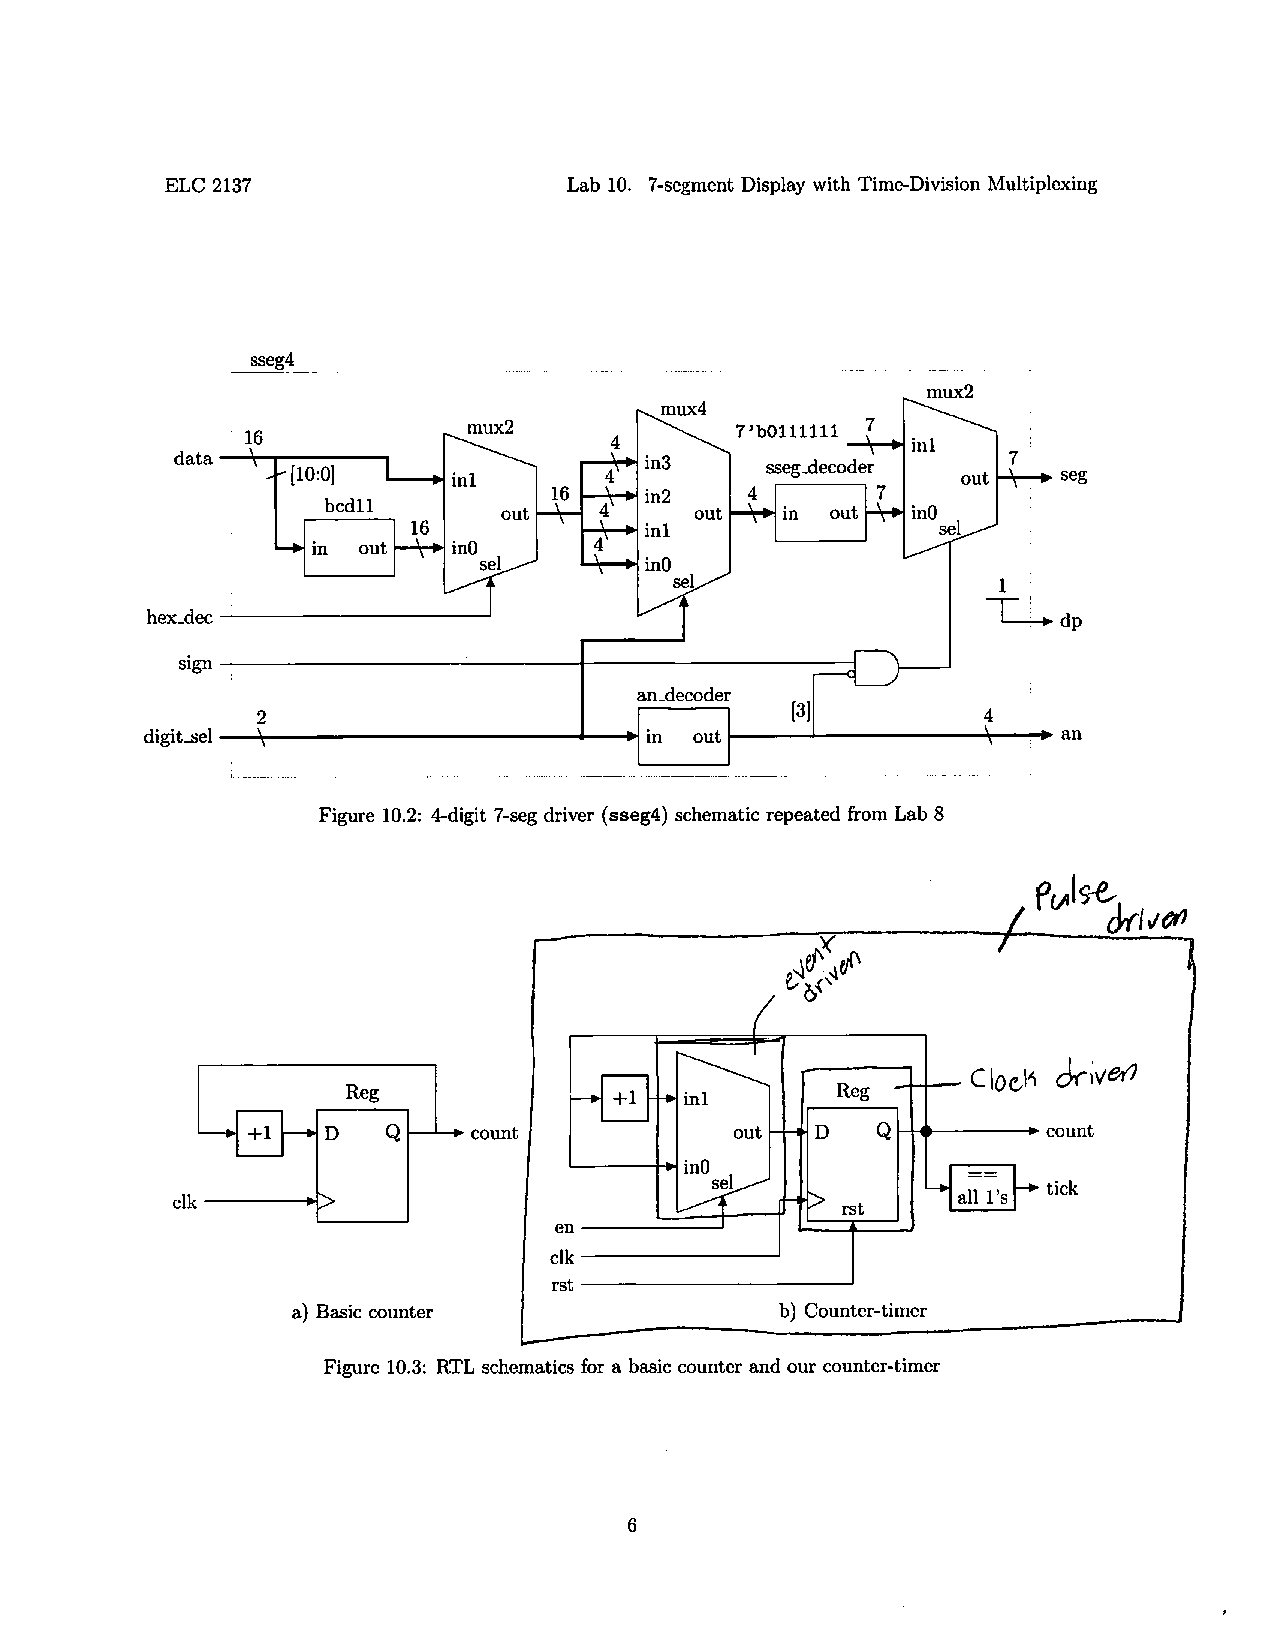
\includegraphics[trim={8.8cm 5cm 0cm 14cm},clip]{10.3_b.pdf}
		\label{fig:picture}
	\end{figure}

	\item If instead of a counter, you wanted to make a shift register that moved the input bits from right to left (low to high). What would you put on the line Q next = /*???*/
	\begin{enumerate}
		\item To make a shift register that moved bits from right to left, you would put on the line Q next = Q reg - 1;
	\end{enumerate}
\end{enumerate}


\clearpage
\section*{Results}

\begin{figure}[ht]\centering
	\begin{tabular}{l|rrrrrrrrrrrrrrrrr}
		Time (ns): & 0 & 20 & 40 & 60 & 80  & 100 & 120 & 140 & 160 & 180 & 200 & 220 & 240 & 260 & 280  & 300 & 320  \\
		\midrule
		clk & 0 & 1 & 1 & 1 & 1 & 1 & 1 & 1 & 1 & 1 & 1 & 1 & 1 & 1 & 1 & 1 & 1 \\
		en & 0 & 1 & 1 & 1 & 0 & 0 & 1 & 0 & 1 & 0 & 1 & 1 & 0 & 1 & 1 & 1 & 1 \\
		rst & 0 & 1 & 0 & 0 & 0 & 0 & 0 & 0 & 0 & 0 & 0 & 0 & 0 & 0 & 0 & 0 & 0 \\
		\midrule
		count & X & 1 & 2 & 3 & 4 & 5 & 6 & 7 & 8 & 9 & a & b & c & d & e & f & 0 \\
		tick & X & 0 & 0 & 0 & 0 & 0 & 0 & 0 & 0 & 0 & 0 & 0 & 0 & 0 & 0 & 1 & 0\\
		\bottomrule
	\end{tabular}\medskip
	
	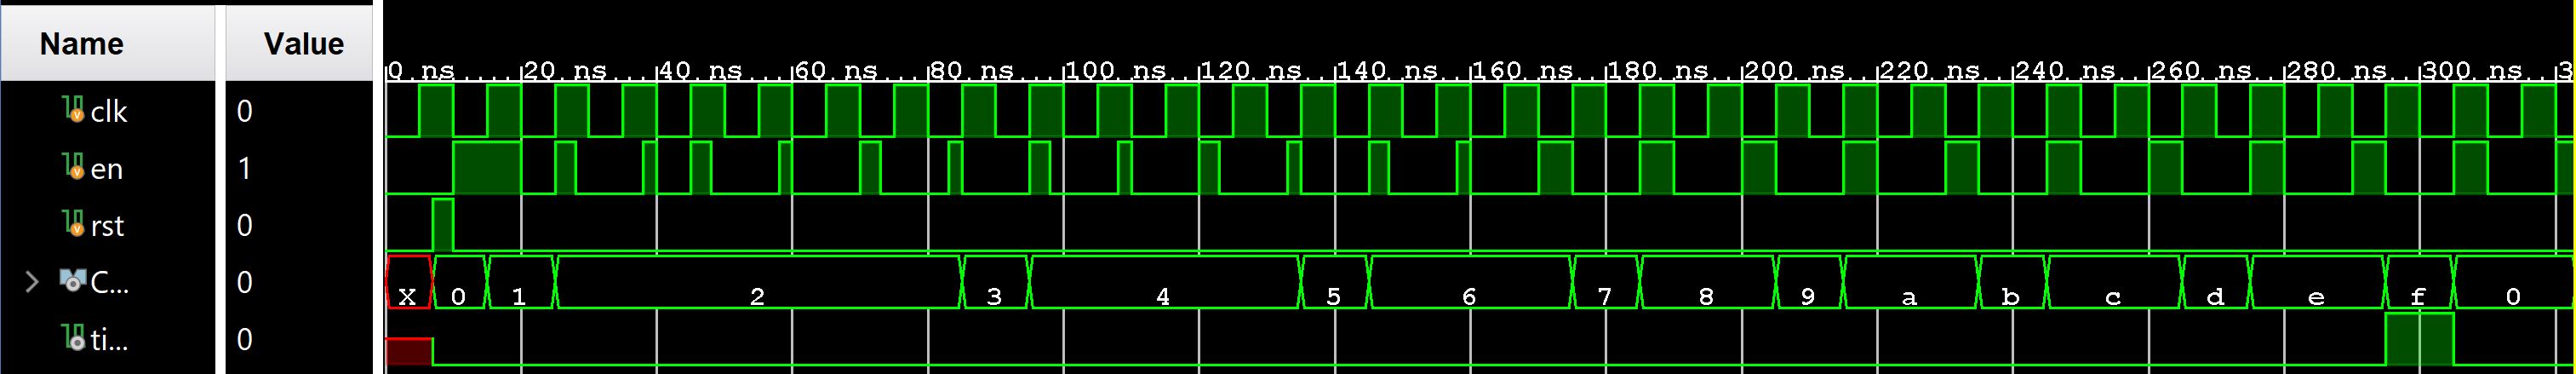
\includegraphics[trim={0cm 0cm 12.5cm 0cm},clip]{Counter_Test.JPG}
	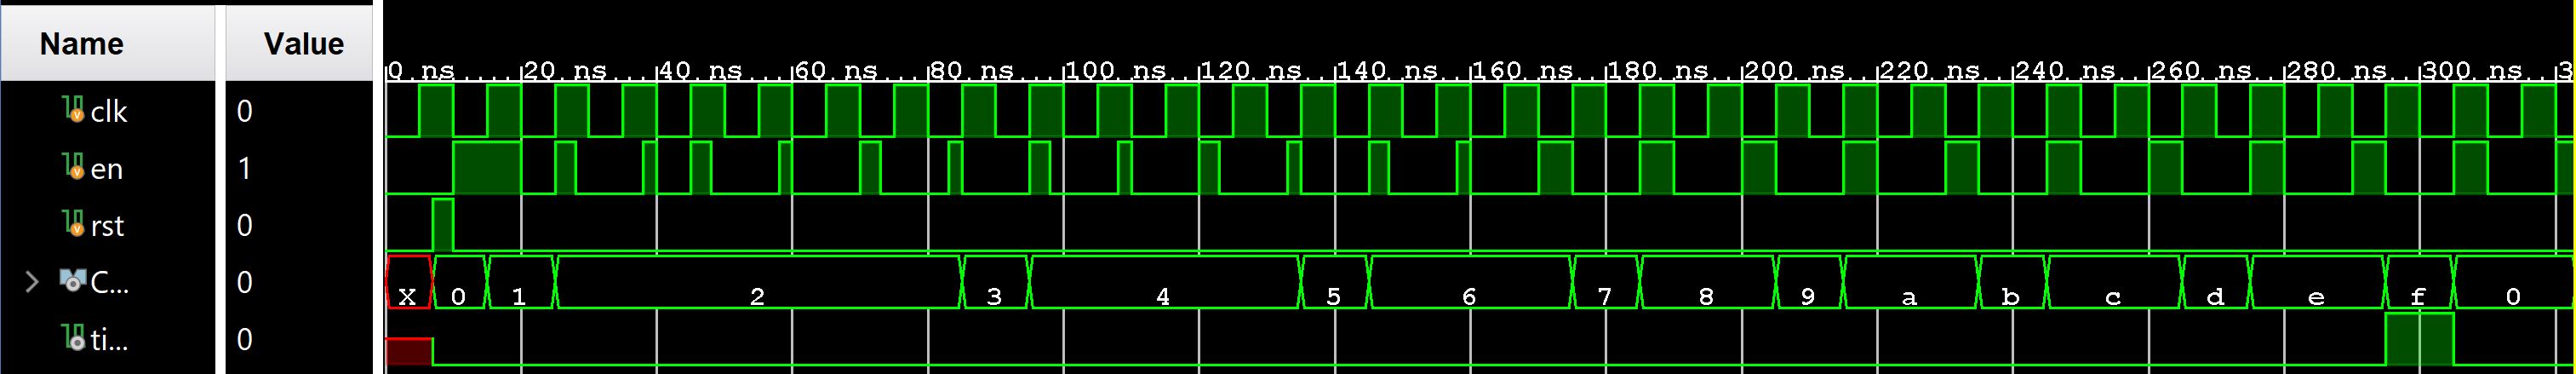
\includegraphics[trim={14cm 0cm 0cm 0cm},clip]{Counter_Test.JPG}
	\caption{Counter simulation waveform and ERT}
	\label{fig:sim_with_table}
\end{figure}

\begin{figure}[ht]\centering
	\begin{tabular}{l|rrrrrrrrrrrrrrrrrrrrr}
		Time (ms): & 0 & 2 & 4 & 6 & 8  & 10 & 12 & 14 & 16 & 18 & 20 & 22 & 24 & 26 & 28  & 30 & 32 & 34 & 36 & 38 & 40  \\
		\midrule
		clk & 0 & 1 & 1 & 1 & 1 & 1 & 1 & 1 & 1 & 1 & 1 & 1 & 1 & 1 & 1 & 1 & 1 & 1 & 1 & 1 & 1 \\
		rst & 1 & 0 & 0 & 0 & 0 & 0 & 0 & 0 & 0 & 0 & 0 & 0 & 0 & 0 & 0 & 0 & 0 & 0 & 0 & 0 & 0 \\
		data & 0 & 1 & 1 & 2 & 3 & 4 & 4 & 5 & 6 & 7 & 8 & 8 & 9 & a & b & c & c & d & e & e & f\\
		hexdec & 0 & 1 & 1 & 1 & 1 & 1 & 1 & 1 & 1 & 1 & 1 & 0 & 0 & 0 & 0 & 1 & 1 & 1 & 0 & 0 & 0 \\
		\midrule
		seg & 40 & 79 & 79 & 24 & 40 & 40 & 40 & 40 & 40 & 40 & 3f & 3f & 30 & 08 & 40 & 79 & 79 & 40 & 40 & 40 & 40\\
		dp & 1 & 1 & 1 & 1 & 1 & 1 & 1 & 1 & 1 & 1 & 1 & 1 & 1 & 1 & 1 & 1 & 1 & 1 & 1 & 1 & 1\\
		an & e & e & e & e & e & d & d & d & 7 & 7 & 7 & e & e & e & d & d & d & b & b & b & 7\\
		\bottomrule
	\end{tabular}\medskip
	
	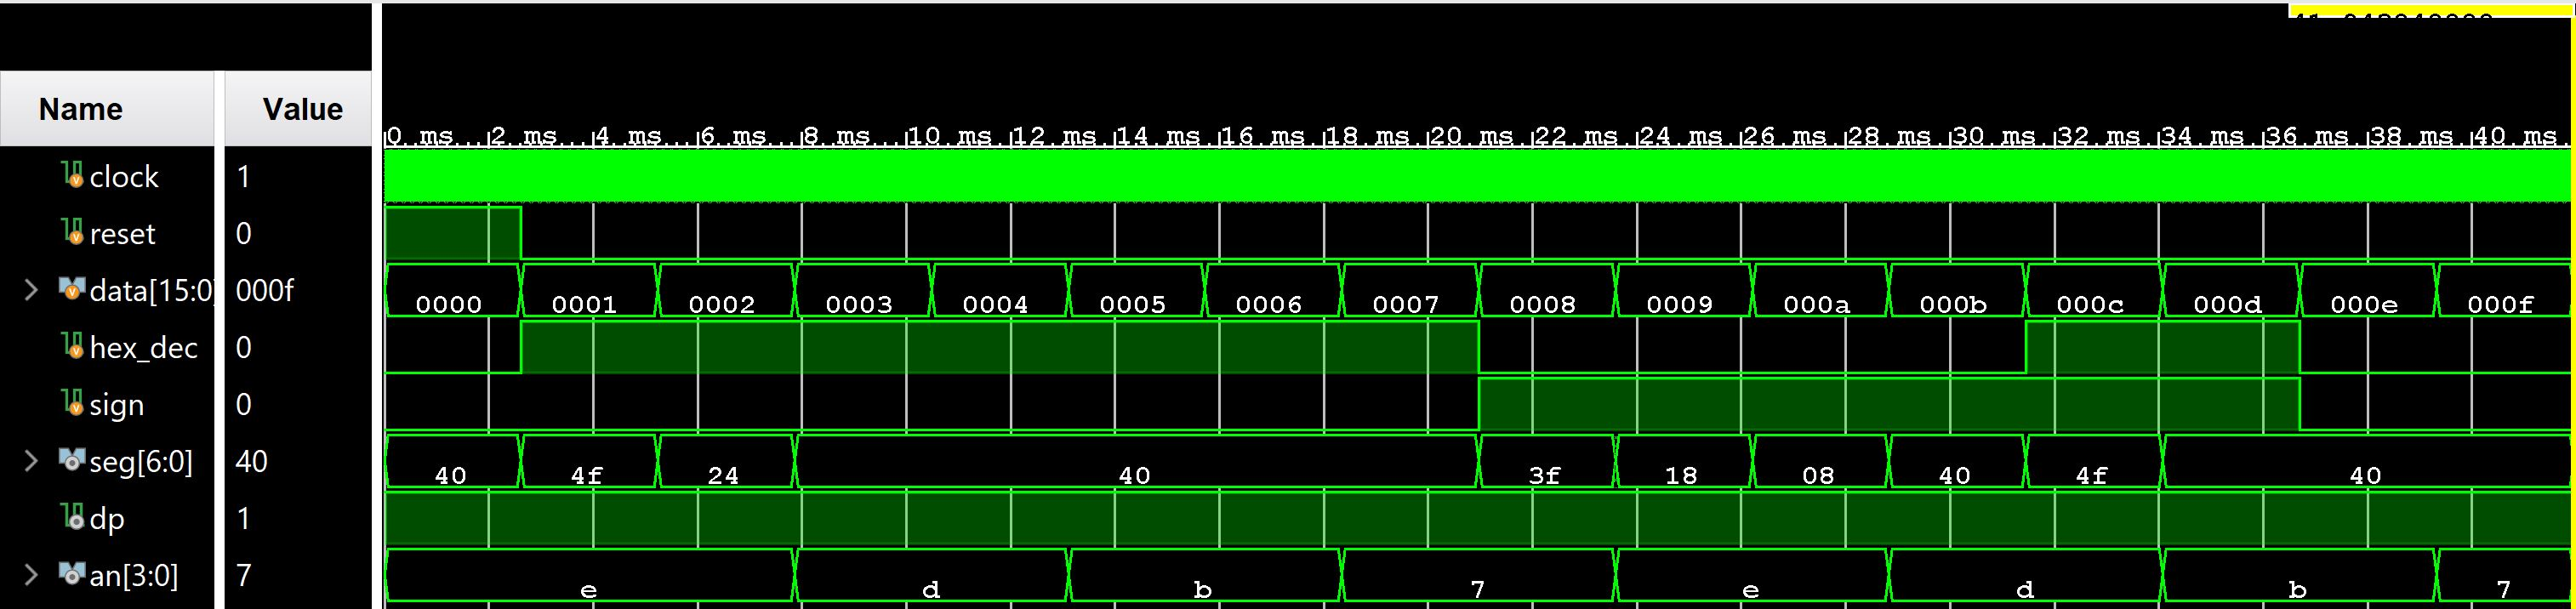
\includegraphics[trim={0cm 0cm 12.5cm 0cm},clip]{sseg4_TDM_Test.JPG}
	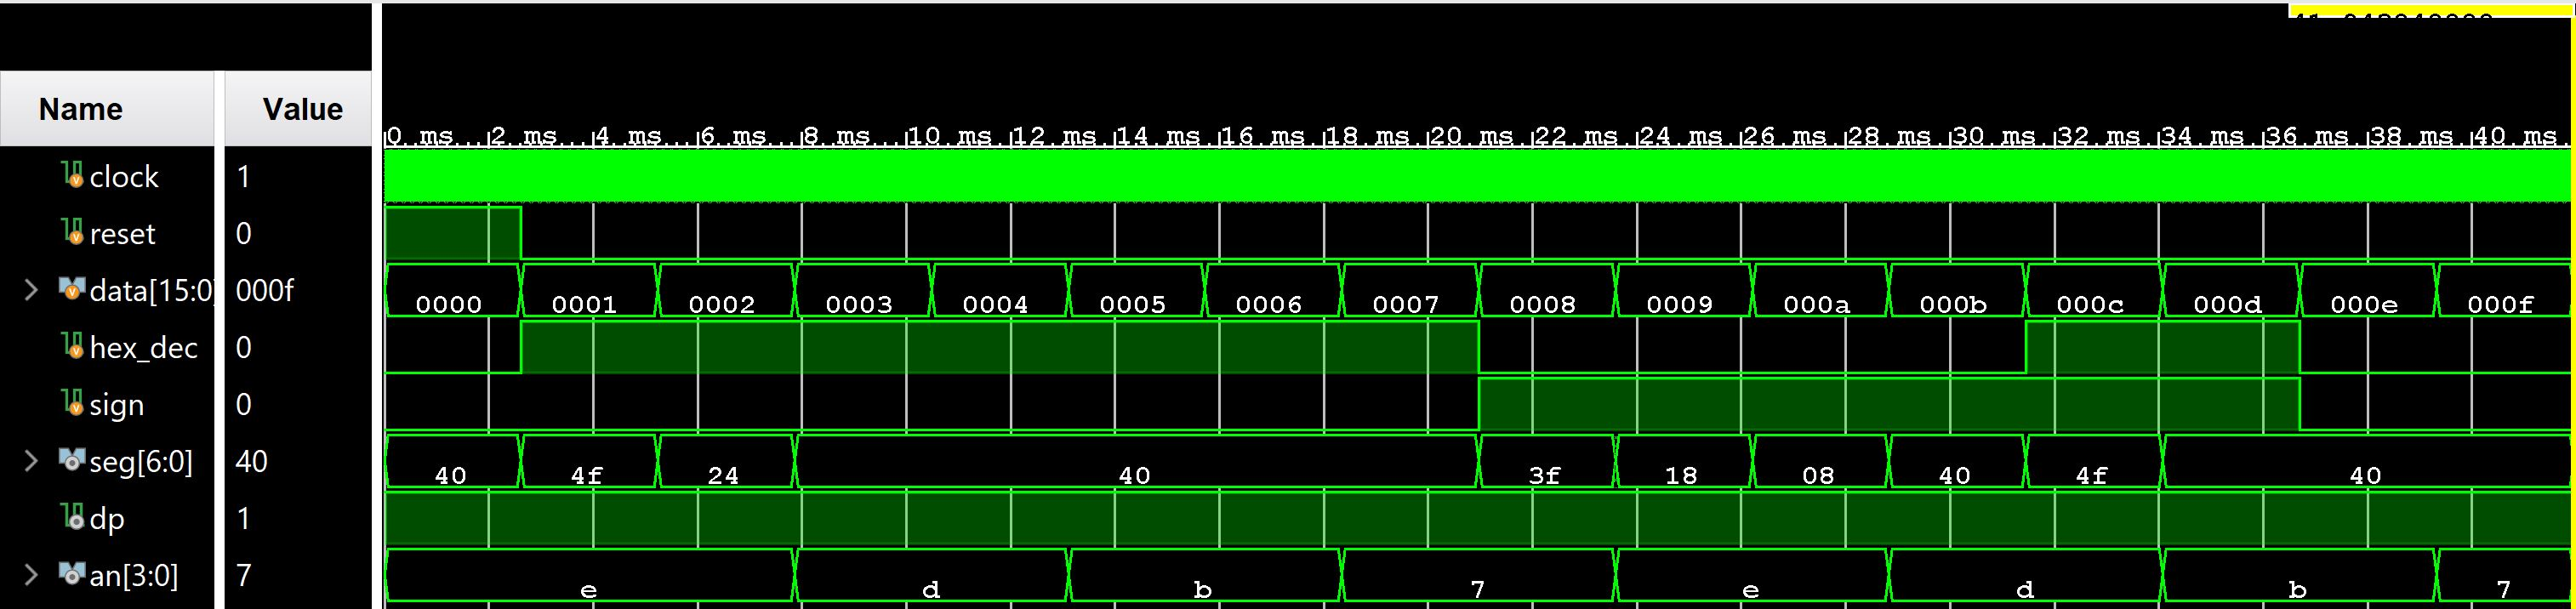
\includegraphics[trim={17.5cm 0cm 0cm 0cm},clip]{sseg4_TDM_Test.JPG}
	\caption{sseg4TDM simulation waveform and ERT}
	\label{fig:sim_with_table}
\end{figure}

\begin{figure}[ht]\centering
	\caption{sseg4TDM Schematic}
	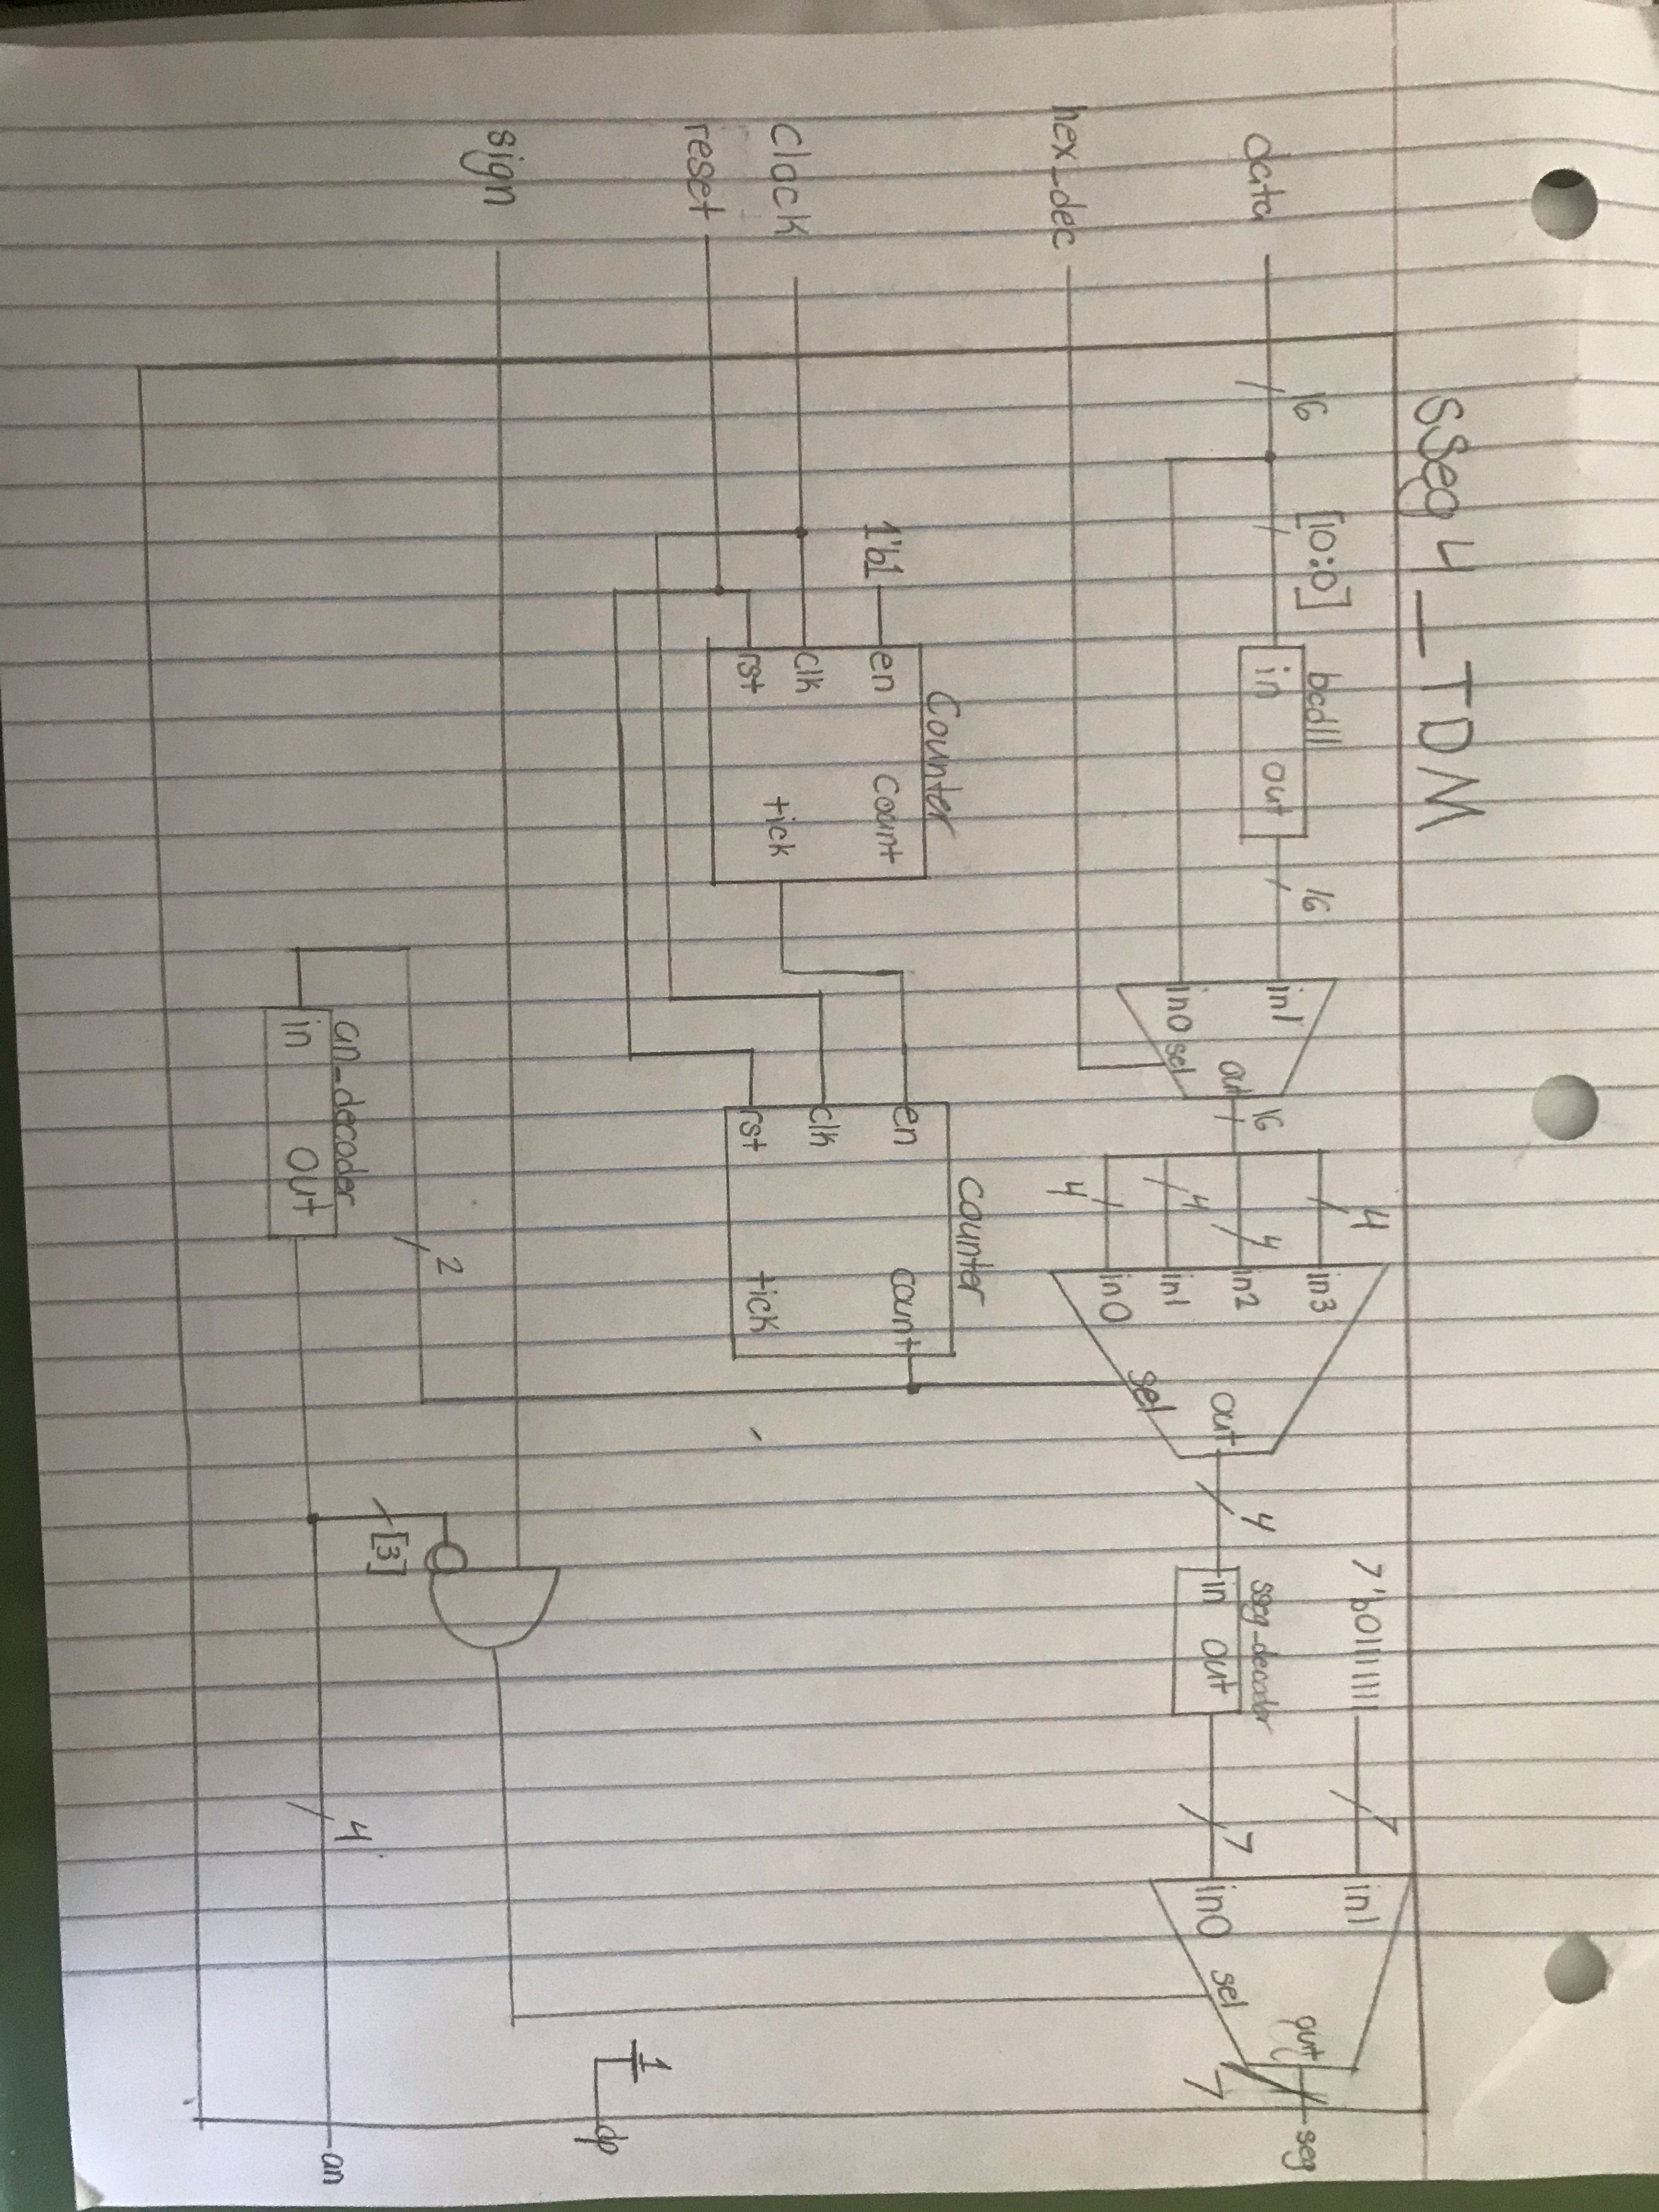
\includegraphics[width=1.05\textwidth]{sseg4_TDM_Schematic.jpeg}
	\label{fig:picture}
\end{figure}

\begin{figure}[ht]\centering
	\caption{calclab10 Schematic}
	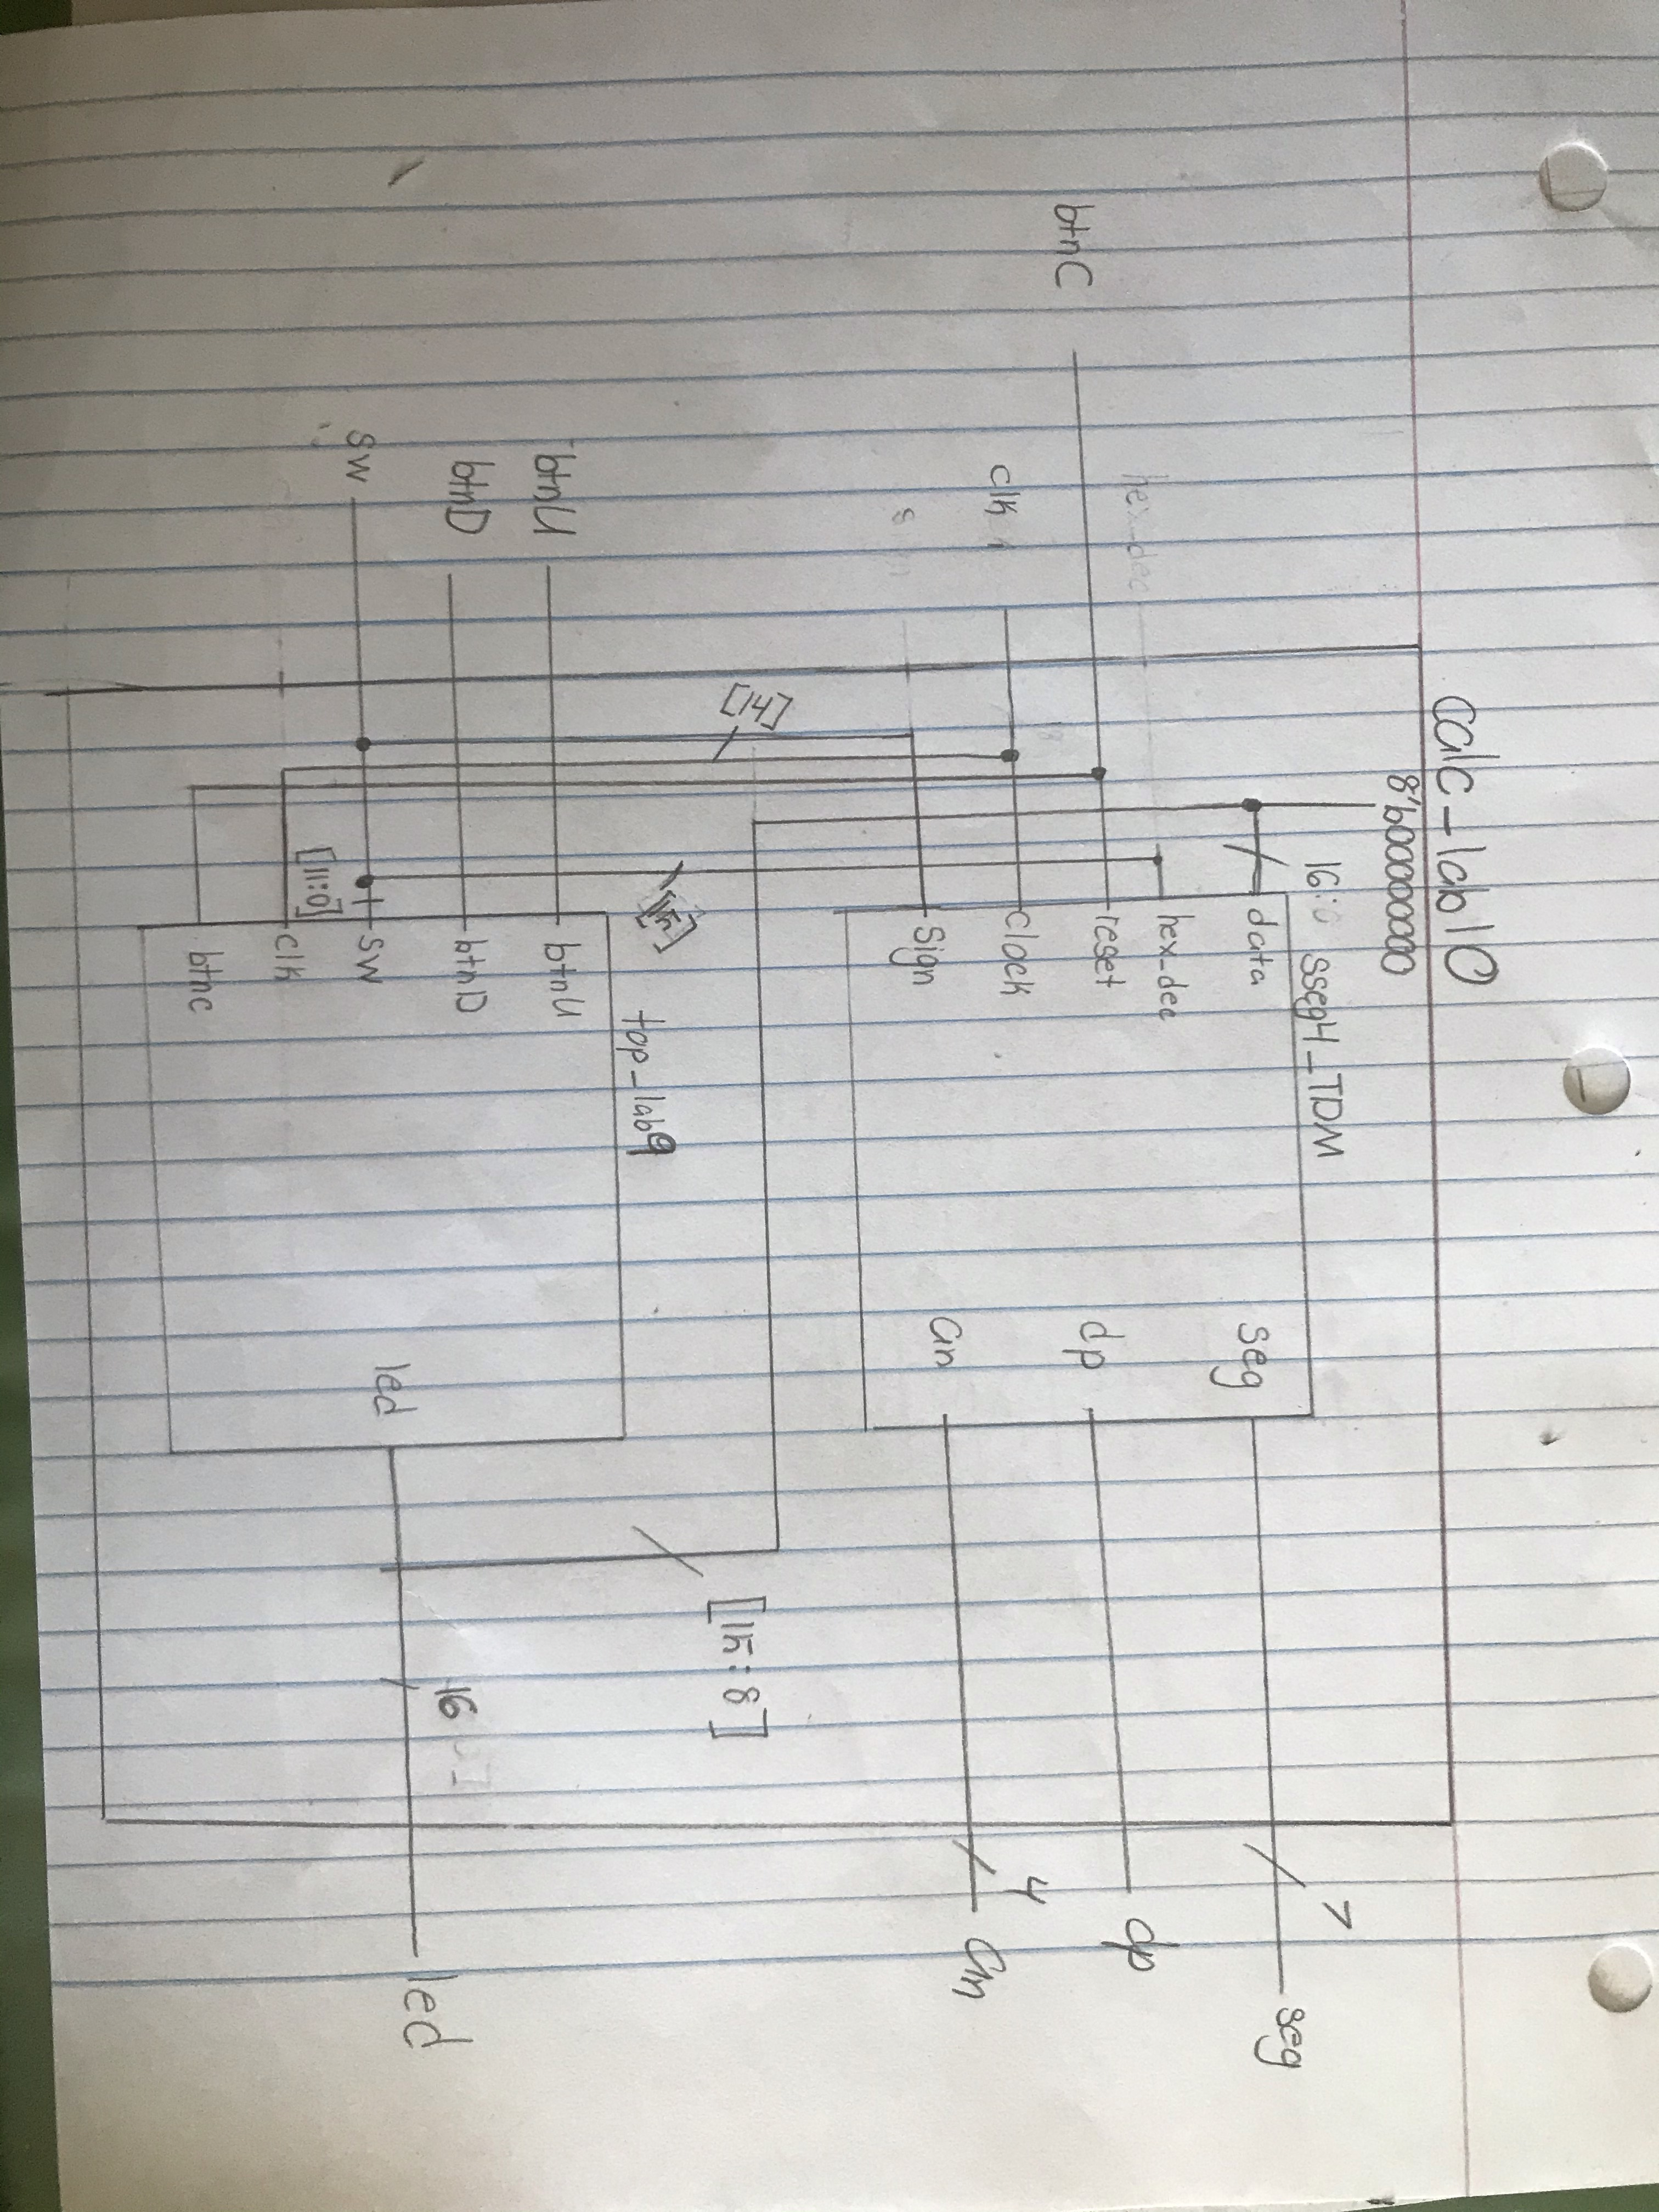
\includegraphics[width=1.15 \textwidth]{calc_lab10_Schematic.jpeg}
	\label{fig:picture}
\end{figure}

\clearpage
\section*{Code}

\begin{lstlisting}[style=Verilog,
caption=Counter Module,
label=counter 
]

`timescale 1ns / 1ps
// ELC 2137 Jake Simmons 2020-7-4

module Counter #(parameter N=1) ( 
	input clk, rst, en, 
	output [N-1:0] count , 
	output tick 
	);
	// internal signals 
	reg [N-1:0] Q_reg , Q_next;
	// register (state memory) 
	always @(posedge clk, posedge rst) 
		begin 
			if (rst) 
				Q_reg <= 0; 
			else 
				Q_reg <= Q_next; 
		end
	// next -state logic 
	always @* 
		begin 
			if (en) 
				Q_next = Q_reg + 1; 
			else 
				Q_next = Q_reg; // no change 
		end
	// output logic 
	assign count = Q_reg; 
	assign tick = (Q_reg=={N{1'b1}}) ? 1'b1 : 1'b0;
	endmodule // counter
\end{lstlisting}

\begin{lstlisting}[style=Verilog,
caption=Counter Test Bench,
label=Counter_test
]
`timescale 1ns / 1ps
//ELC 2137 Jake Simmons 2020-7-4

module counter_test();
	reg clk, en, rst; 
	wire [3:0] count;
	wire tick;

	Counter #(.N(4)) count1( .tick(tick), .clk(clk), 

	.en(en), .rst(rst), .count(count) );



	// clock runs continuously 

	always begin 

		clk = ~clk; #5; 

	end

	// this block only runs once 

	initial begin

		clk = 0; en = 0; rst = 0; #7;
		rst = 1; #3; // reset 
		en = 1; rst = 0; #10; 
		en = 0; #5; 
		en = 1; #3;
		en = 0; #10; 
		en = 1; #2; 
		en = 0; #5; 
		en = 1; #3;
		en = 0; #10; 
		en = 1; #2; 
		en = 0; #10; 
		en = 1; #3; 
		en = 0; #10; 
		en = 1; #2; 
		en = 0; #10; 
		en = 1; #3; 
		en = 0; #10; 
		en = 1; #2; 
		en = 0; #10; 
		en = 1; #3; 
		en = 0; #10; 
		en = 1; #2; 
		en = 0; #10; 
		en = 1; #3; 
		en = 0; #10; 
		en = 1; #2; 
		en = 0; #10; 
		en = 1; #3;
		en = 1; #2; 
		en = 0; #10; 
		en = 1; #3; 
		en = 1; #2; 
		en = 0; #10; 
		en = 1; #3; 
		en = 1; #2; 
		en = 0; #10; 
		en = 1; #3; 
		en = 1; #2; 
		en = 0; #10; 
		en = 1; #3; 
		en = 1; #2; 
		en = 0; #10; 
		en = 1; #3; 
		en = 1; #2; 
		en = 0; #10; 
		en = 1; #3; 
		en = 1; #2; 
		en = 0; #10; 
		en = 1; #3; 
		en = 1; #2; 
		en = 0; #10; 
		en = 1; #3; 
		en = 1; #2; 
		en = 0; #10; 
		en = 1; #3; 
		en = 1; #2; 
		en = 0; #10; 
		en = 1; #3; 

	$finish;

	end
endmodule

\end{lstlisting}

\begin{lstlisting}[style=Verilog,
caption=sseg4TDM Module,
label=sseg4TDM
]
`timescale 1ns / 1ps
//ELC 2137 2020-4-7

module sseg4_TDM(
	input clock,
	input reset,
	input [15:0] data,
	input hex_dec,
	input sign,
	output [6:0] seg,
	output dp,
	output [3:0] an
	);
	
	wire [1:0] digit_sel;    
	wire [15:0] W1 ;
	wire [15:0] W2 ;
	wire [3:0] W3;
	wire [6:0] W4;
	wire [3:0] W5;
	wire W6;    
	wire [1:0] W7;

	Counter #(.N(18)) timer( .clk(clock), .en(1'b1), .tick(W7), .rst(reset));  
	
	Counter #(.N(2)) counter2( .clk(clock),.en(W7),.count(digit_sel), .rst(reset) );   
	  
	BCD11_2 B1( .in11(data[10:0]), .out11(W1));
	
	mux2 #(.N(16)) B2( .in0(data), .in1(W1), .sel(hex_dec), .out(W2));
	
	mux4 B3( .in0(W2[3:0]), .in1(W2[7:4]), .in2(W2[11:8]), .in3(W2[15:12]), .sel(digit_sel), .out(W3));
	
	sseg_decoder B5( .num(W3), .sseg(W4));
	
	mux2 #(.N(7)) B6( .in0(W4), .in1(7'b0111111), .out(seg) , .sel(W6));
	
	and G2( W6, sign, ~W5[3]);
	
	annode_decoder B7( .in(digit_sel), .out(W5));

	assign dp = 1;
	assign an = W5;
endmodule


\end{lstlisting}

\begin{lstlisting}[style=Verilog,
caption=sseg4TDM Test Bench,
label=sseg4TDM Test
]
`timescale 1ns / 1ps
//ELC 2137 2020-7-4

module sseg4_TDM_test();
	reg clock;
	reg reset;
	reg [15:0] data;
	reg hex_dec;
	reg sign;
	wire [6:0] seg;
	wire dp;
	wire [3:0] an;

	sseg4_TDM sseg4( .clock(clock), .reset(reset), .data(data), .hex_dec(hex_dec),
	.sign(sign), .seg(seg), .dp(dp), .an(an));



	// clock runs continuously 

	always begin 

		clock = ~clock; #10; 

	end

	// this block only runs once 

	initial begin
		data = 0; hex_dec = 0; reset = 1;  clock = 0; sign = 0; #2621440;
		data = 1; hex_dec = 1; reset = 0;  sign = 0; #2621440;
		data = 2; hex_dec = 1; reset = 0;  sign = 0;  #2621440;
		data = 3; hex_dec = 1; reset = 0;  sign = 0;  #2621440;
		data = 4; hex_dec = 1; reset = 0;  sign = 0;  #2621440;
		data = 5; hex_dec = 1; reset = 0;  sign = 0;  #2621440;
		data = 6; hex_dec = 1; reset = 0;  sign = 0;  #2621440;
		data = 7; hex_dec = 1; reset = 0;  sign = 0;  #2621440;
		data = 8; hex_dec = 0; reset = 0;  sign = 1;  #2621440;
		data = 9; hex_dec = 0; reset = 0;  sign = 1;  #2621440;
		data = 10; hex_dec = 0; reset = 0;  sign = 1;  #2621440;
		data = 11; hex_dec = 0; reset = 0;  sign = 1;  #2621440;
		data = 12; hex_dec = 1; reset = 0;  sign = 1;  #2621440;
		data = 13; hex_dec = 1; reset = 0;  sign = 1;  #2621440;
		data = 14; hex_dec = 0; reset = 0;  sign = 0;  #2621440;
		data = 15; hex_dec = 0; reset = 0;  sign = 0;  #2621440;

	$finish;

	end
endmodule


\end{lstlisting}

\begin{lstlisting}[style=Verilog,
caption=calclab10 Module,
label=calclab10
]

`timescale 1ns / 1ps
//ELC 2137 Jake Simmons 2020-4-8

module calc_lab10(
	input clk,
	input btnU,
	input btnD,
	input [11:0] sw,
	input btnC,
	output [15:0] led,
	output [6:0] seg,
	output dp,
	output [3:0] an
	);
	wire [7:0] W1;

	sseg4_TDM disp_unit( .data({8'b00000000, W1}), .hex_dec(sw[15]),
	.reset(btnC), .clock(clock), .sign(sw[14]), 
	.seg(seg), .dp(dp), .an(an));

	top_lab9 calc_unit( .btnU(btnU), .btnD(btnD), .sw(sw[11:0]),
	.clk(clk), .btnC(btnC), .led(led) );

	assign w1 = led[15:8];
endmodule


\end{lstlisting}


\end{document}
